
%(BEGIN_QUESTION)
% Copyright 2014, Tony R. Kuphaldt, released under the Creative Commons Attribution License (v 1.0)
% This means you may do almost anything with this work of mine, so long as you give me proper credit

Fyll ut verditabellen for denne kretsen:

$$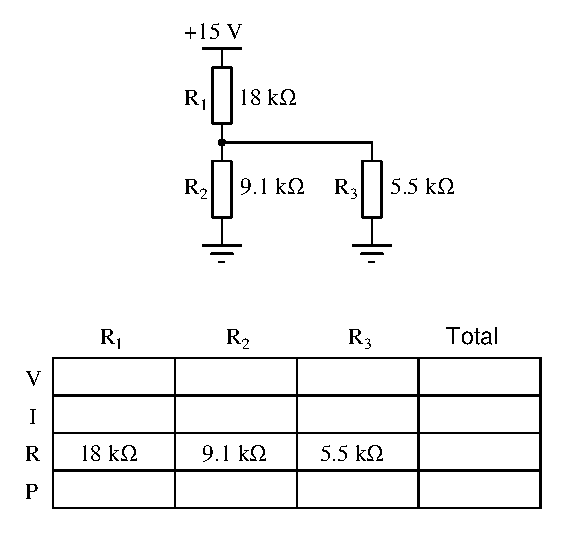
\includegraphics[width=15.5cm]{i01169x01.eps}$$

\underbar{file i01169}
%(END_QUESTION)





%(BEGIN_ANSWER)

$$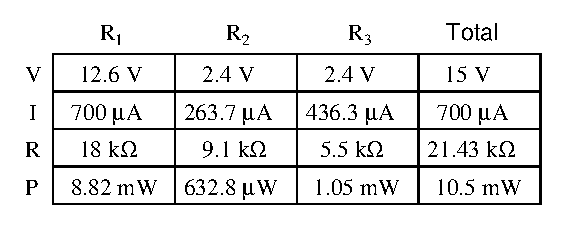
\includegraphics[width=15.5cm]{i01169x02.eps}$$

%(END_ANSWER)





%(BEGIN_NOTES)

Et viktig trekk ved dette koblingsskjemaet er hvordan strømforsyningstilkoblingene er vist.  I motsetning til mange andre skjemaer bruker jeg ikke et ``batteri''-symbol for spenningskilden her.  I stedet vises forsynings-``rail''-symboler (en flat linje og et jordsymbol).  Gjør elevene oppmerksomme på at dette er svært vanlig symbolbruk i moderne skjemaer, og at det i praksis sparer oss for å tegne ledninger til en spenningskilde (og selve kildesymbolet).

\vskip 10pt

Diskuter med elevene hva som kan være en god framgangsmåte for å beregne de ukjente verdiene i denne oppgaven, og hvordan de kan kontrollere arbeidet sitt.

\vskip 10pt

Elever har ofte vansker med å formulere en løsningsmetode: hvilke trinn de skal ta for å gå fra gitte betingelser til et endelig svar.  Det er nyttig at du (læreren) viser dette i starten, men det er uheldig å gjøre det for ofte, fordi elevene da kan slutte å tenke selv og bare følge oppskriften din.  En undervisningsteknikk jeg har hatt god nytte av, er å la elever komme opp til tavla (alene eller i grupper) og skrive løsningsstrategiene sine slik at alle kan se dem.  De trenger ikke regne ut alt, men kan skissere trinnene de ville fulgt, i riktig rekkefølge.

Når elevene \underbar{skisserer løsningsstrategiene sine}, får alle se flere måter å løse oppgaven på, og du (læreren) får innsikt i hvordan, og om, elevene faktisk tenker.  Et spesielt viktig punkt i slike ``åpen tenkning''-aktiviteter er hvordan man kontrollerer arbeidet sitt for å avdekke feil.

%INDEX% Elektronikkrepetisjon: serie-parallellkretser

%(END_NOTES)
